\documentclass[17pt]{report}
\usepackage[utf8]{inputenc}
\usepackage{amsmath}
\usepackage{graphicx}
\usepackage{hyperref}
\usepackage{listings}
\usepackage{color}
\hypersetup{
    colorlinks=true,
    linkcolor=blue,
    filecolor=magenta,      
    urlcolor=cyan,
}
 
\urlstyle{same}
\definecolor{codegreen}{rgb}{0,0.6,0}
\definecolor{codegray}{rgb}{0.5,0.5,0.5}
\definecolor{codepurple}{rgb}{0.58,0,0.82}
\definecolor{backcolour}{rgb}{0.95,0.95,0.92}
\lstdefinestyle{mystyle}{
    backgroundcolor=\color{backcolour},   
    commentstyle=\color{codegreen},
    keywordstyle=\color{magenta},
    numberstyle=\tiny\color{codegray},
    stringstyle=\color{codepurple},
    basicstyle=\footnotesize,
    breakatwhitespace=false,         
    breaklines=true,                 
    captionpos=b,                    
    keepspaces=true,                 
    numbers=left,                    
    numbersep=5pt,                  
    showspaces=false,                
    showstringspaces=false,
    showtabs=false,                  
    tabsize=2
}
\lstset{style=mystyle}
\graphicspath{ {../Images/} }
\title{
	{\large Statistical learning: Second assignment}\\}
\author{Ali Zamani(96123035)}
\begin{document}
\maketitle

\newpage
\section{Import packages}
\lstinputlisting[language=python, firstline=1, lastline=13]{../pythonCode/TensorFlow.py}
\section{Load Data Set:}
In this section we define function loadDataSet for loading data.Inputs of this function are:\\
1)directory: address of data set file.\\
2)trainNum:  number of training data.\\
3)validNum:  number of validation data.\\
\lstinputlisting[language=python, firstline=14, lastline=36]{../pythonCode/TensorFlow.py}
\section{Define variables , constants and placeholders of the logistic regression model}
First we set epochNum=5000 , batchSize=500 , trainNum=3500 ,validNum=100 and learningRate=1e-6 for 
maximum likelihood and 1e-6 for binary cross-entropy and regularized binary cross-entropy. \\
Deta set was loded by calling the  loadDataSet function.\\
we must define to placeholders, one of them for input(named as x) and another one for output(named as y).\\
Two variables w and b are also defined.\\
\lstinputlisting[language=python, firstline=37, lastline=54]{../pythonCode/TensorFlow.py} 
\section{Define logistic regression model, loss functions and optimizers}
ypredicted was defined for modeling.\\
Three loss functions lossML, lossBCE, lossRBCE were also defined for maximum likelihood, binary cross-entropy and regularized binary cross-entropy.\\
Gradient Descent Optimizer was used for optimizing.\\
\lstinputlisting[language=python, firstline=55, lastline=66]{../pythonCode/TensorFlow.py} 
\section{Run Session}
We run the session for three different loss functions ans report the results.
\lstinputlisting[language=python, firstline=67, lastline=91]{../pythonCode/TensorFlow.py} 
\section{Results}
\lstinputlisting[language=python, firstline=92, lastline=110]{../pythonCode/TensorFlow.py} 
maximum likelihood:\\\\\\\\
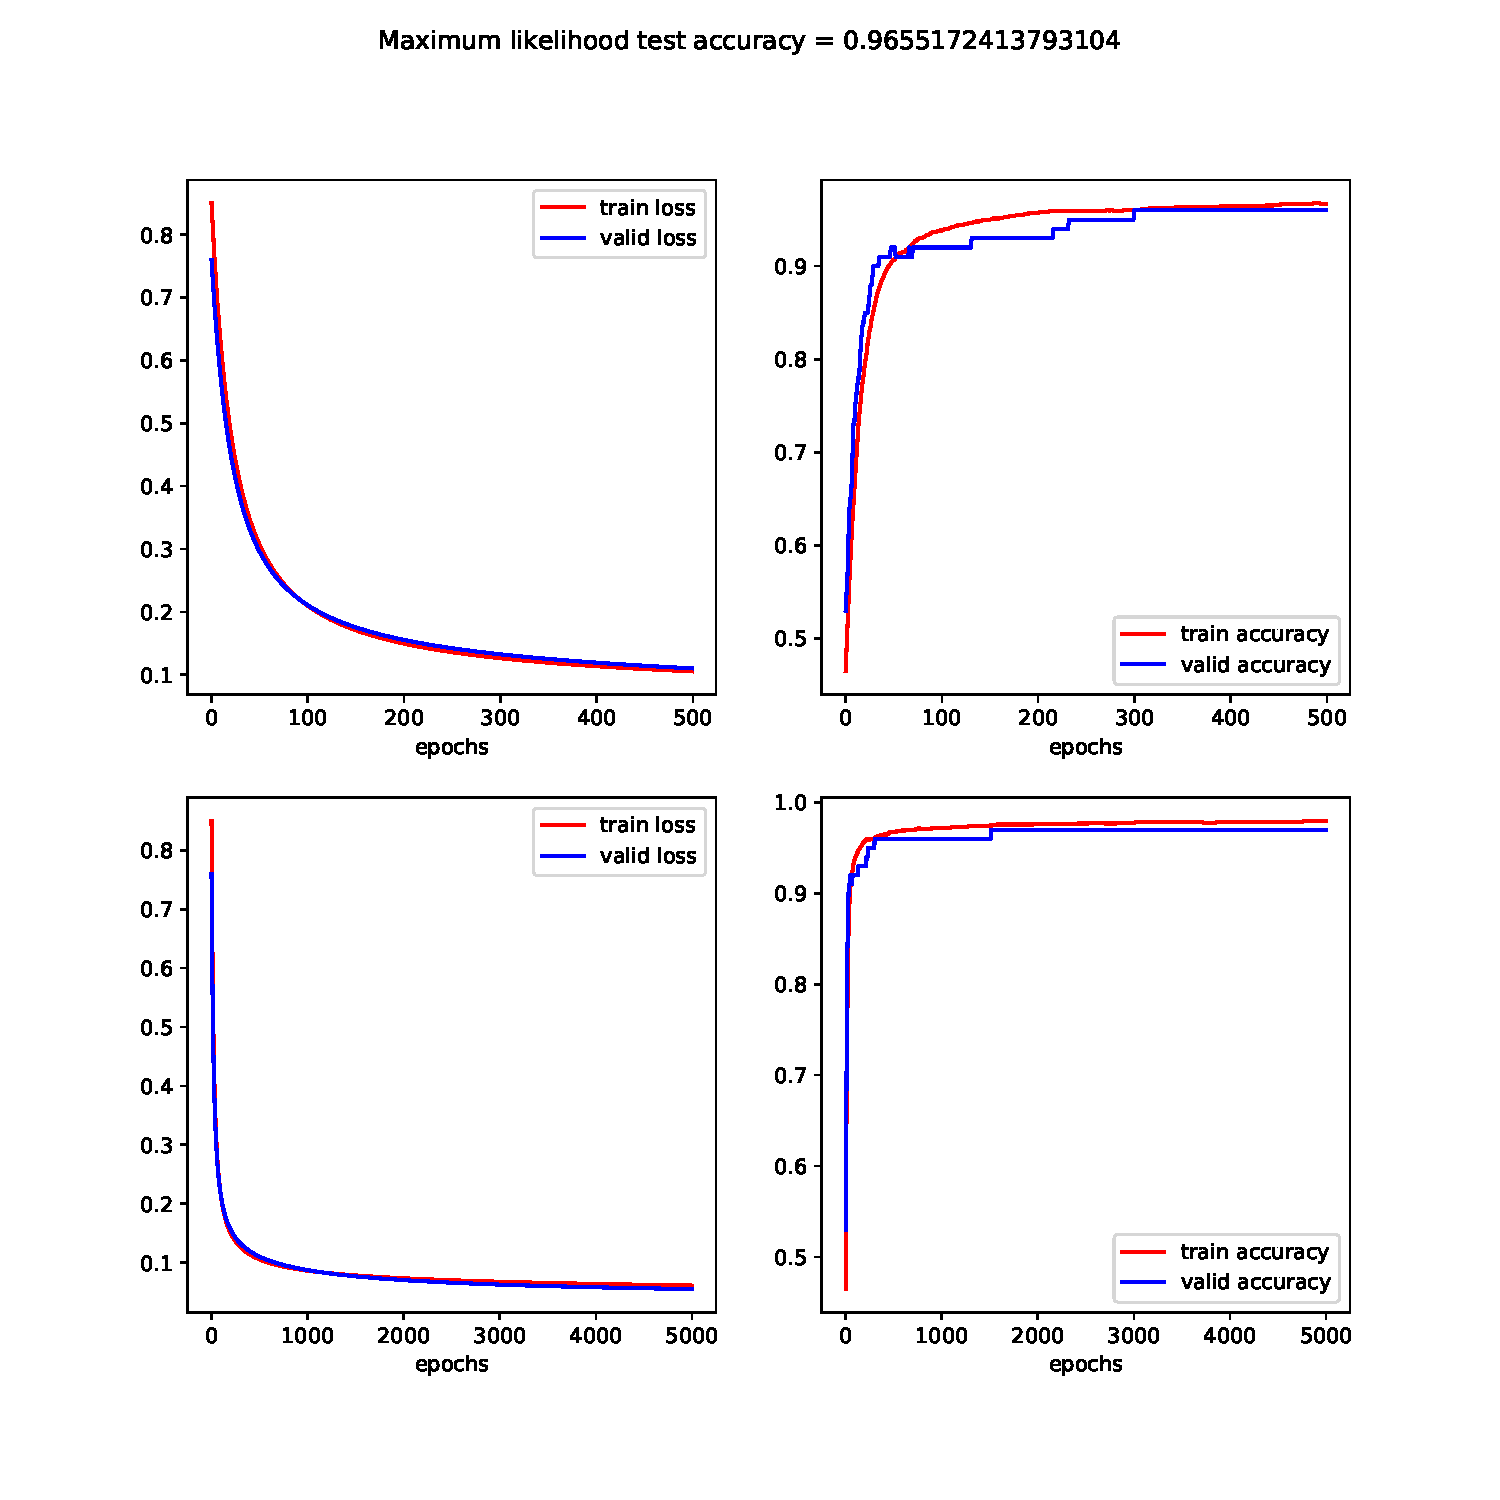
\includegraphics[width=12cm, height=10cm]{ML}\\\\
binary cross-entropy:\\\\\\
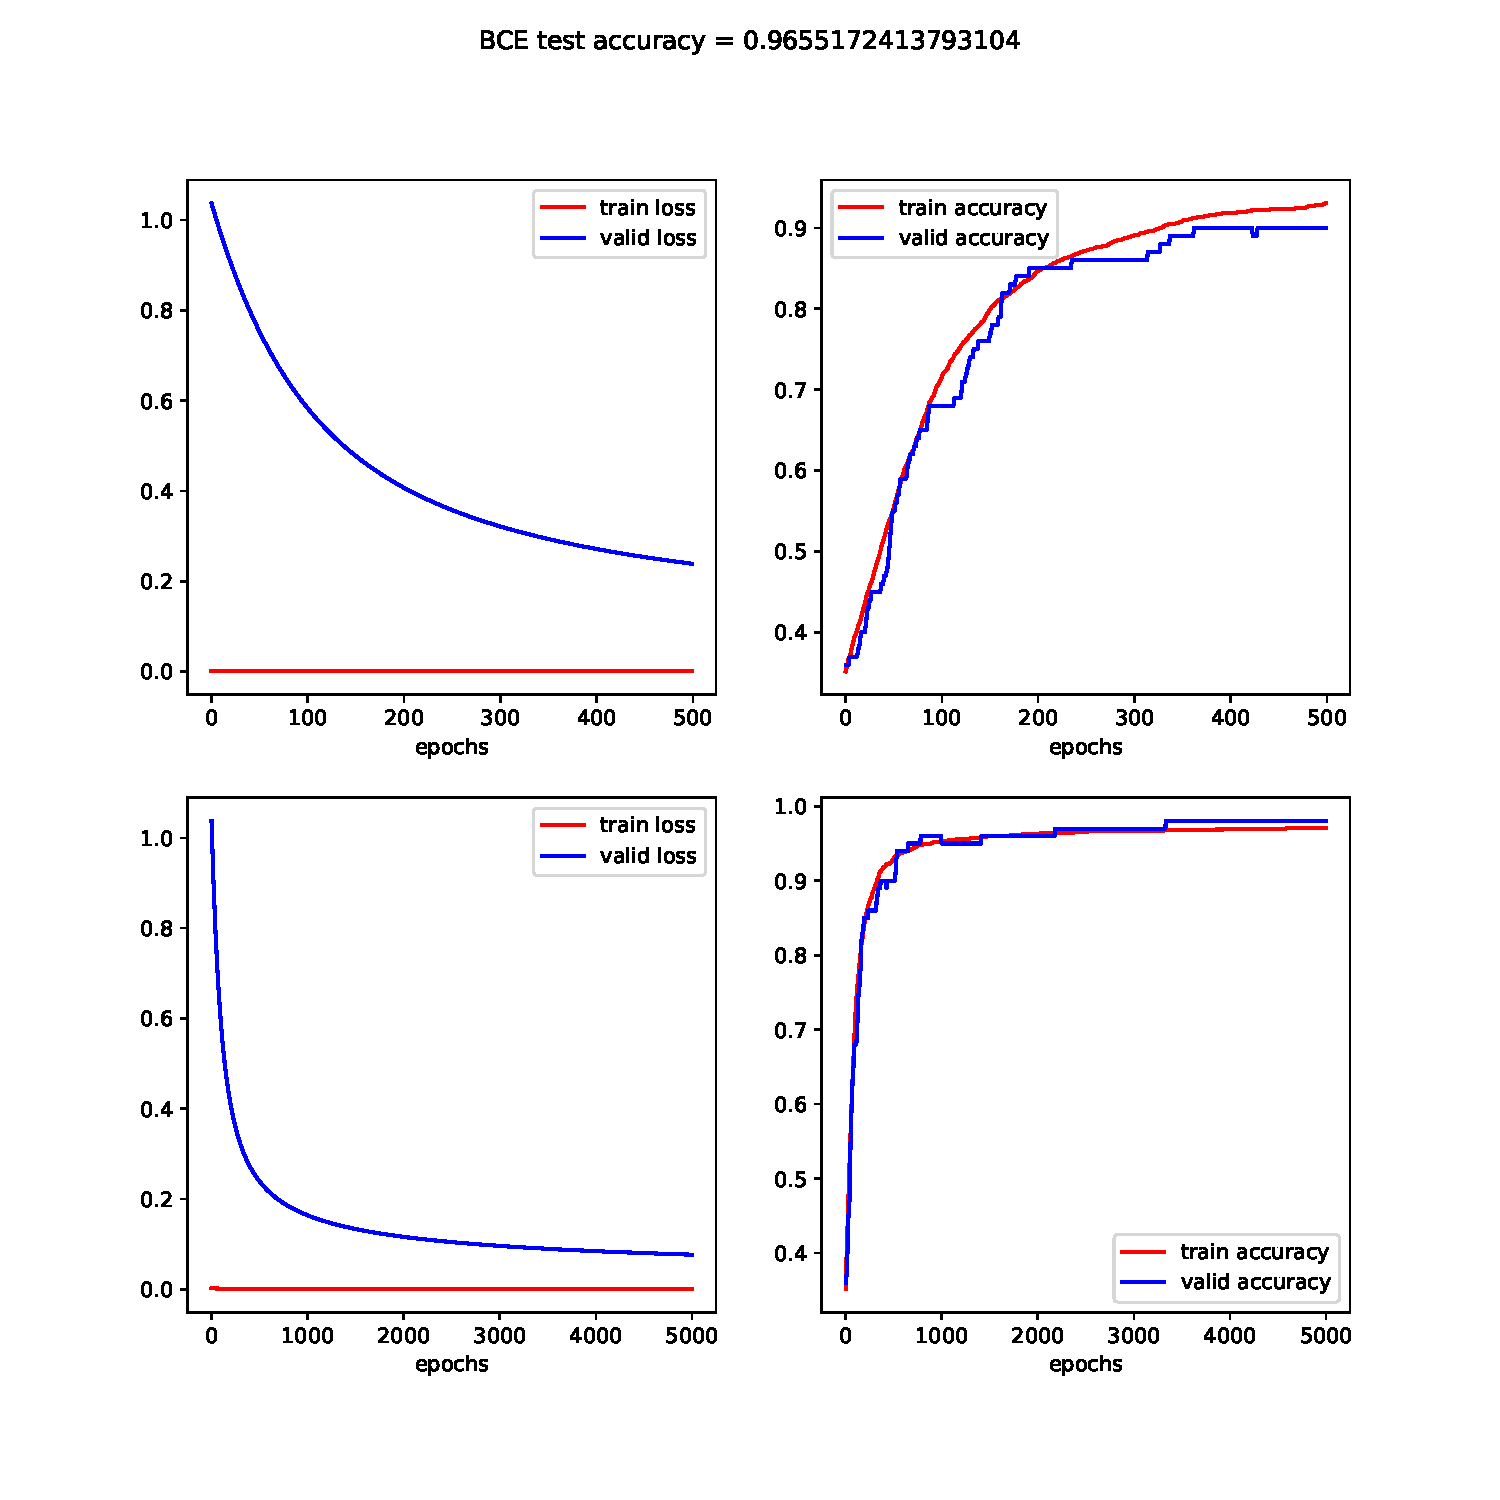
\includegraphics[width=15cm, height=15cm]{BCE}\\\\\\\\\\\\\\\\
regularized binary cross-entropy:\\\\\\\\
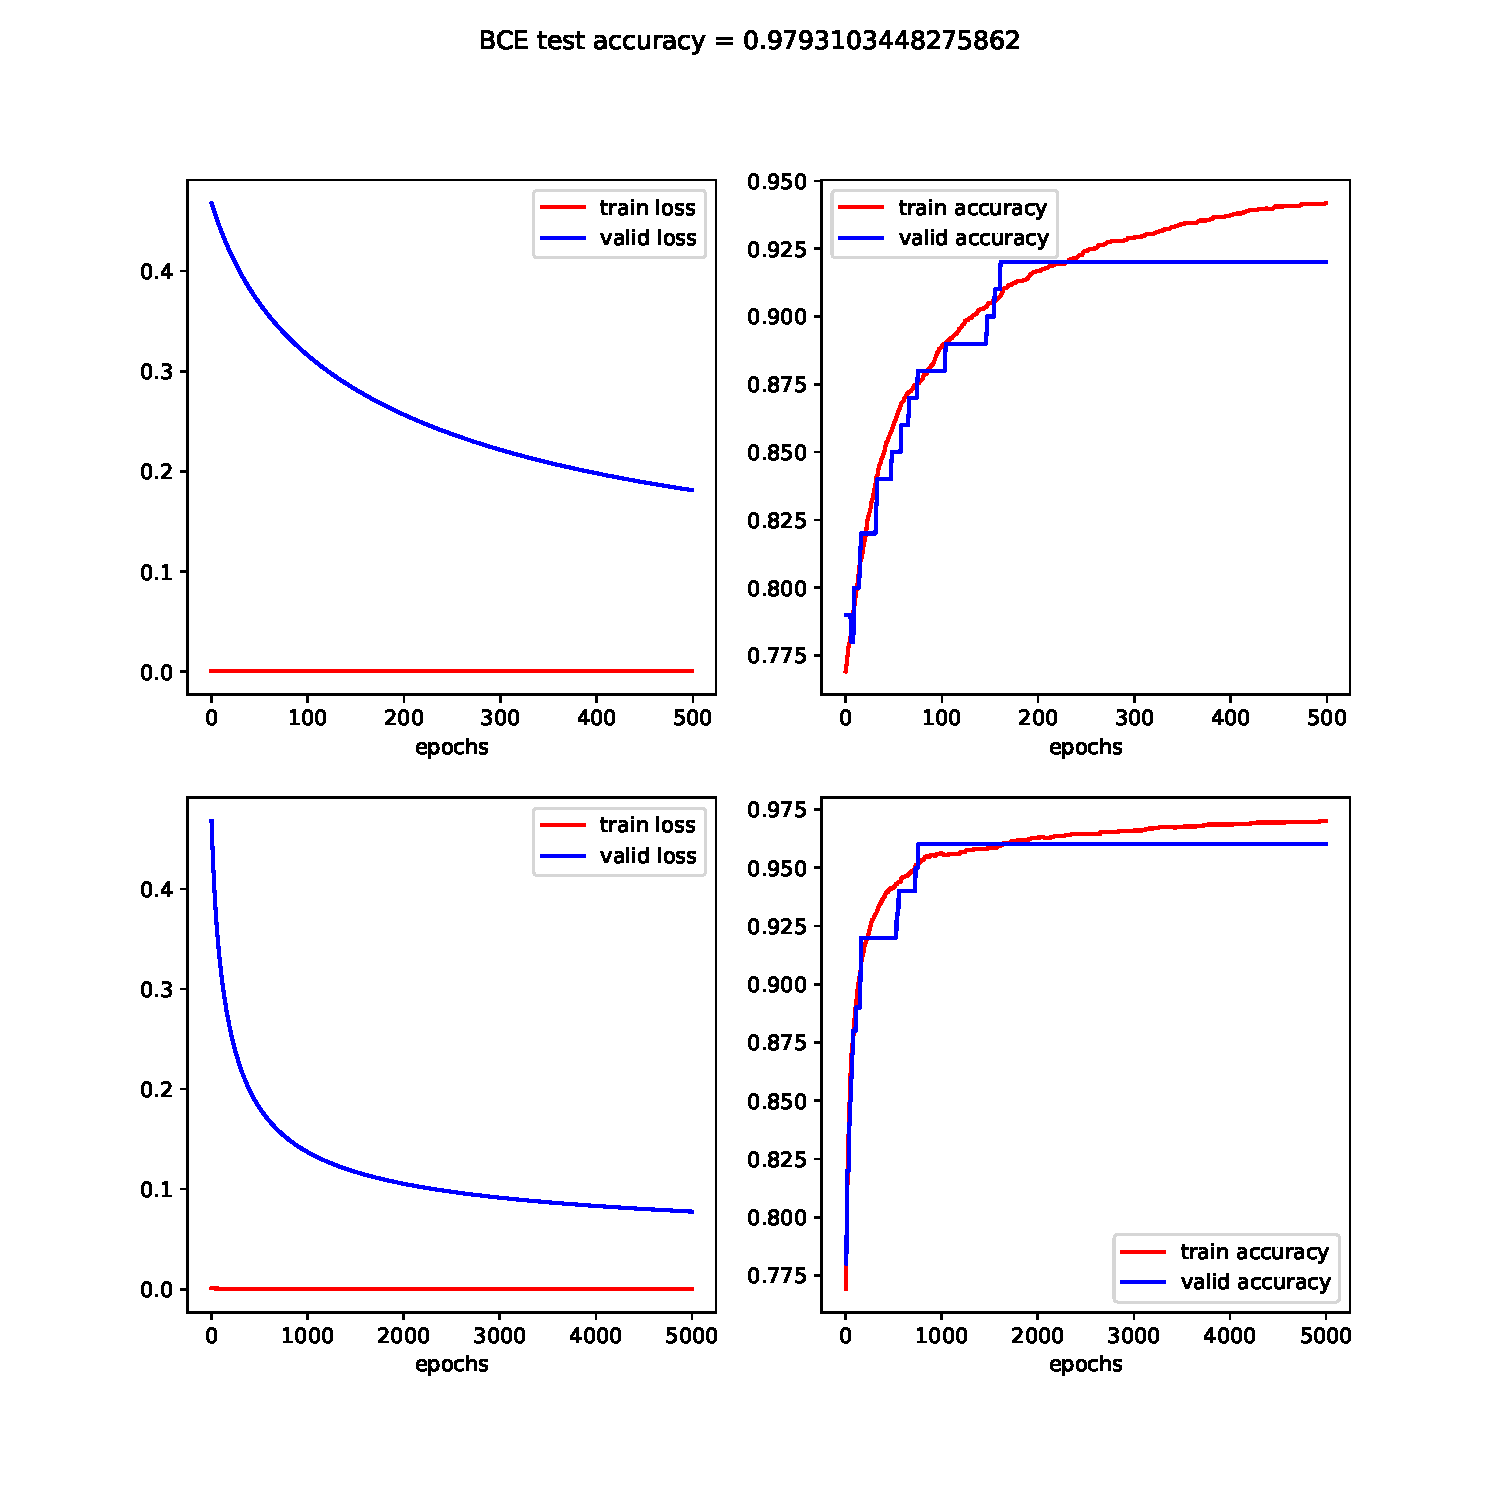
\includegraphics[width=15cm, height=15cm]{RBCE}\\
\href{https://github.com/zamaniali1995/Linear-Regressions-and-Linear-Models-using-the-Iris-Data}{Source Code}
\end{document}